\chapter{Types and Interfaces}

In this chapter, we give an overview of the fundamental 
data structures and definitions used in the library.
These sections contains type definitions.
Type definitions are what differentiate TS from JS.
With them, we are able to precisely define what properties objects have.

However, before we get into this chapter,
it is useful to understand some of the naming conventions
that will be used.
Class, types and interface definitions follow \mintinline{ts}{PascalCase}.
Local variables, instance variables,
and getters follow \mintinline{ts}{snake_case}.
Functions follow \mintinline{ts}{camelCase}.

In this chapter, we will take a look at the most basic
types and interfaces:
\mintinline{ts}{base_id}, \mintinline{ts}{VertexArgs},
\mintinline{ts}{EdgeArgs}, \mintinline{ts}{NetworkArgs}.
And we will also describe the basic structure of the \mintinline{ts}{Vertex},
\mintinline{ts}{Edge}, and \mintinline{ts}{Network} classes.

These type definitions are the foundation of the library.
They are stored inside \mintinline{ts}{enums.ts}.

The \mintinline{ts}{base_id} type is used throughout in the library.
It signifies that the identification variable for a vertex can be either
a string of characters or a number.

\begin{minted}[bgcolor=bg]{typescript}
export type base_id = string | number;
\end{minted}

Given a vertex in a graph, it is necessary to assign an ID.
This helps us identify what vertex we are are refering to when we
want to do certain operations or calculations with the vertex.
The type \mintinline{ts}{string | number} means that the ID of an vertex
can be a string such as \mintinline{ts}{"vertex_a"}or a number such as 42.

\begin{minted}[bgcolor=bg]{typescript}
export interface VertexArgs {
  id: base_id;
  weight?: number;
}
\end{minted}

The \mintinline{ts}{Args} interfaces are used by function inputs.
For example, when creating an edge,
the library will be expecting an object with the format of \mintinline{ts}{EdgeArgs}.

The question-mark indicates a property is optional.
Weights are optional parameters, and set to one by default.
This means that, on a technical level, all networks are weighted.
The difference between an unweighted network and a weighted one
is that the weighted network contains weights other than one.
Edges, just like vertices, also have IDs.

Because NeTS doesn't deal with multigraphs, we
could have gone without edge IDs.
This architecture is an example of how NeTS
has been prepared with the possibility of dealing
with multigraphs.

\begin{minted}[bgcolor=bg]{typescript}
export interface EdgeArgs {
  from: base_id;
  to: base_id;
  id?: base_id;
  weight?: number;
  do_force?: boolean;
}
\end{minted}

Notice that all properties of \mintinline{ts}{NetworkArgs} are optional.
Therefore, it is possible to create a network without using any parameters.
The following is an example of code that creates a network \mintinline{ts}{net},
adds the vertices `1' and `b' to it, and an edge between them.
It is visually represented in Figure \ref{fig:net_1b}.

\begin{minted}[bgcolor=bg]{typescript}
export interface NetworkArgs {
  is_directed?: boolean;
  edge_limit?: number;
  vertex_limit?: number;
}
\end{minted}

Here is how we could go about creating a network:

\begin{minted}[bgcolor=bg]{typescript}
const net = new Network()

net.addVertex({ id: 1 })
net.addVertex({ id: 'b' })

net.addEdge(1, 'b')
\end{minted}

The functions \mintinline{ts}{addEdge()} and \mintinline{ts}{addVertex()}
are explained in the Functions section.

\begin{figure}[H]
  \centering
  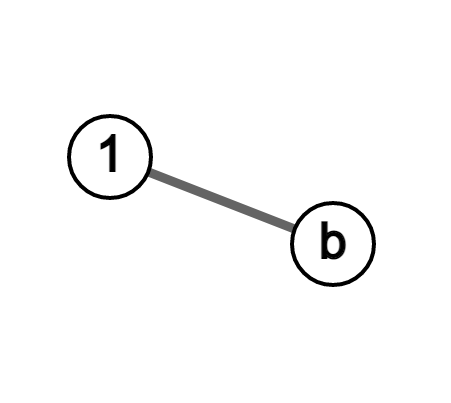
\includegraphics[scale=.25]{img/ex_net_1b.png}
  \caption{`net' with an edge between `1' and `b'.}
  \label{fig:net_1b}
\end{figure}

Networks are by default undirected.
A directed network has to be explicitly declared.
In the following code, we create a directed network,
and add an edge that connects `1' to `b'.

\begin{minted}[bgcolor=bg]{typescript}
const is_directed = true
const directed_net = new Network({ is_directed })
directed_net.addEdge(1, 'b')
\end{minted}

Notice that adding an edge automatically adds the nodes associated with it.
This behavior is related to the \mintinline{ts}{do_force} property and
is further discussed in the Functions section.

\begin{figure}[H]
  \centering
  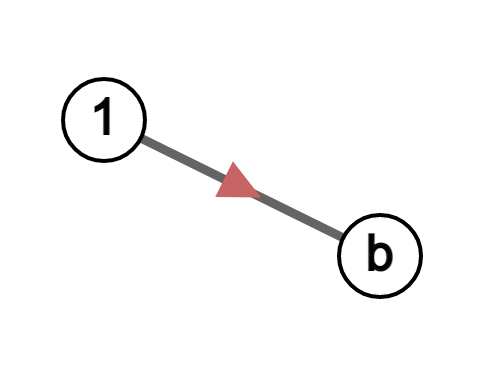
\includegraphics[scale=.25]{img/ex_net_1b_dir.png}
  \caption{A directed edge from `1' to `b'}
  \label{fig:net_1b_dir}
\end{figure}

\mintinline{ts}{ParsedCSV} and \mintinline{ts}{ERROR} are types used internally
by the library to load CSV files and manage error messages, respectively.
NeTS features for reading and writing CSV files are very useful for
analyzing network data.
A very common way of storing the information of a network is
through an adjacency matrix.
Adjacency matricies are most often written into a CSV file.
For example because NeTS has the ability to read adjacency matrices,
it is possible to import a network that was created elsewhere
and use it with the library.

\begin{minted}[bgcolor=bg]{typescript}
export type ParsedCSV = string[][];

export const ERROR = {...};
\end{minted}

\section{Vertex and Edge Classes}

In this chapter, we will see the two base classes used by NeTS:
\mintinline{ts}{Vertex} and \mintinline{ts}{Edge}.

The vertex class receives an object with the interface of \mintinline{ts}{VertexArgs}.
The weight is optional and set to 1 if not provided as a parameter.

\begin{minted}[bgcolor=bg]{typescript}
import { base_id, VertexArgs } from "./enums.ts";

export class Vertex {
  readonly id: base_id;
  weight: number;

  constructor(args: VertexArgs) {
    this.id = args.id;
    this.weight = args.weight ?? 1;
  }
}
\end{minted}

The \mintinline{ts}{??} operator is a `Nullish coalescing operator,' introduced in ES2021.
If \mintinline{ts}{args.weight} is undefined, the instruction on the right is chosen.
This operator is used instead of the ternary \mintinline{ts}{a ? b : c} operator
because, if \mintinline{ts}{args.weight = 0},
\mintinline{ts}{??} would still select \mintinline{ts}{args.weight},
whereas the ternary operator would consider `0' a Falsy value.

A Falsy value is something with the same Boolean value as false.
For example, `0', although a number, is still considered Falsy in TS and in JS.
In other languages, such as Ruby, `0' actually has a Truthy value,
meaning that if you feed it into a logical operation, it evaluates to true.

The edge class has \mintinline{ts}{from} and \mintinline{ts}{to} properties that hold
the ID of one vertex each, and a weight.
The IDs of the vertices in an edge are private,
meaning they cannot be read or overwritten.
When an edge is added to a network, only its weight can be altered from outside the class.
Its two vertices and ID cannot be changed. 

Changing the vertices of an edge would fundamentally change what that edge is and is thus not allowed.
The vertices can be accessed and read through the \mintinline{ts}{vertices} getter,
which returns the edge's \mintinline{ts}{from} and \mintinline{ts}{to} properties:

\begin{minted}[bgcolor=bg]{typescript}
import { base_id, EdgeArgs } from "./enums.ts";

export class Edge {
  private to: base_id;
  private from: base_id;
  weight: number;

  constructor(args: EdgeArgs) {
    this.from = args.from;
    this.to = args.to;
    this.weight = args.weight ?? 1;
  }

  /**
   * Returns an object with the two vertices in the edge.
   * @returns {{ from:base_id, to:base_id }}
   */
  get vertices(): { from: base_id; to: base_id } {
    return { from: this.from, to: this.to };
  }
}
\end{minted}

\section{Network Constructor}

The network class has 4 \mintinline{ts}{readonly} properties.
The edges and vertices are stored in Maps that use \mintinline{ts}{base_id},
as their keys and the values store the actual vertex or edge instance.
The two other \mintinline{ts}{readonly} properties are booleans that store fundamental graph properties:
the directionality and complexity of the network.

The \mintinline{ts}{private} properties have to do with hidden functionality
and performance limitations.

There are limits to the number of edges and vertices a network can have,
and in NeTS they can only be set in the creation of a network.
NeTS sets those limits to be \mintinline{ts}{edge_limit=500} and \mintinline{ts}{vertex_limit=500}
by default.
Most of the time when it is necessary to work with a graph data structure,
the scale of such graphs is already known.
Therefore, to assist with error handling limits to the number of edges and vertices are set.
This helps because it prevents users from getting into infinite loops that try to add
too many edges or vertices.

Note the \mintinline{ts}{is_multigraph} property.
Recall that in the introduction we mentioned that although multigraphs
are beyond the scope of the capstone, the library was setup so
as to allow for multigraph support in the future.
The \mintinline{ts}{is_multigraph} is such an example of ``future-proofing''.

\begin{minted}[bgcolor=bg]{typescript}
class Network {
  readonly edges: Map<base_id, Edge>;
  readonly vertices: Map<base_id, Vertex>;

  readonly is_directed: boolean;
  readonly is_multigraph: boolean;

  private edge_limit: number;
  private vertex_limit: number;
  private free_eid: number;
  private free_vid: number;

  constructor(args: NetworkArgs = {}) {
    this.edges = new Map();
    this.vertices = new Map();
    this.is_directed = args.is_directed ?? false;
    this.edge_limit = args.edge_limit ?? 500;
    this.vertex_limit = args.vertex_limit ?? 500;
    this.free_eid = 0;
    this.free_vid = 0;
    this.is_multigraph = false;
  }
}
\end{minted}

Note that, although there are many properties being set 
in the \mintinline{ts}{Network} class constructor,
they are all optional, and have defaults in case the user does not provide them.
The \mintinline{ts}{free_eid} and \mintinline{ts}{free_vid} properties will be further explained later.
A network with a larger number of maximum edges and vertices could be created as such:

\begin{minted}[bgcolor=bg]{typescript}
const edge_limit = 10_000
const vertex_limit = 10_000

const net = new Network({ edge_limit, vertex_limit })
\end{minted}